\section{Example of a LaTeX document}

\subsection{Introduction}

\begin{definition}{Definition Title}\\
    This is a definition.
\end{definition}

\begin{concept}{Concept Title}\\
    This is a concept.
\end{concept}

\begin{lemma}{Lemma Title}\\
    This is a lemma.
\end{lemma}

\begin{theorem}{Theorem Title}\\
    This is a theorem.
    \begin{itemize}
        \item This is an item.
        \item This is another item.
    \end{itemize}
\end{theorem}

\begin{corollary}{Corollary Title}\\
    This is a corollary.
    \begin{enumerate}
        \item This is an enumerated item.
        \item This is another enumerated item.
    \end{enumerate}
\end{corollary}

\begin{example}
    this is a simple example. no title required.
\end{example}

\begin{example2}{Example Title}\\
    this is a more complex example. title required.
\end{example2}

\begin{example2}{Example Title}\\
    One can achieve better readability by seperating the task definition (exercise)
    \tcblower
    from the solution (solution).
\end{example2}

\subsubsection{Code and Formulas}

\begin{code}{Code Title}\\
    This is a code block, where general concepts are explained.
\begin{lstlisting}[language=Java, style=basesmol]
// Indentation matters in these blocks, so all the way to the left!
def example_function(param1, param2):
    // This is a comment
    return param1 + param2
\end{lstlisting}
\end{code}

\begin{examplecode}{Example Code Title}\\
    This is an example code block. This should show specific implementations or examples.
\begin{lstlisting}[language=Python, style=basesmol]
# Indentation matters in these blocks, so all the way to the left!
def example_function(param1, param2):
    # This is a comment
    return param1 + param2
\end{lstlisting}
\end{examplecode}

\begin{formula}{Formula Title}\\
  This is a formula.
  $$E = mc^2$$
  This should be used for very important formulas and concepts. 
\end{formula}

\begin{KR}{KR Title}\\
    This is a KR. This "Kochrezept" is a recipe for a specific exercise type. It should be used for very important recipes and concepts.
    \paragraph{First step}
    This is the first step of the recipe.
    \paragraph{Second step}
    and so on.
\end{KR} 

\subsection{Special Cases}

\begin{definition}{Definition Title}
    \begin{itemize}
        \item this is an itemized list
    \end{itemize}
    if after a title there is a list, no need to add a new line manually.
\end{definition}

\begin{definition}{Definition Title}
    \\
    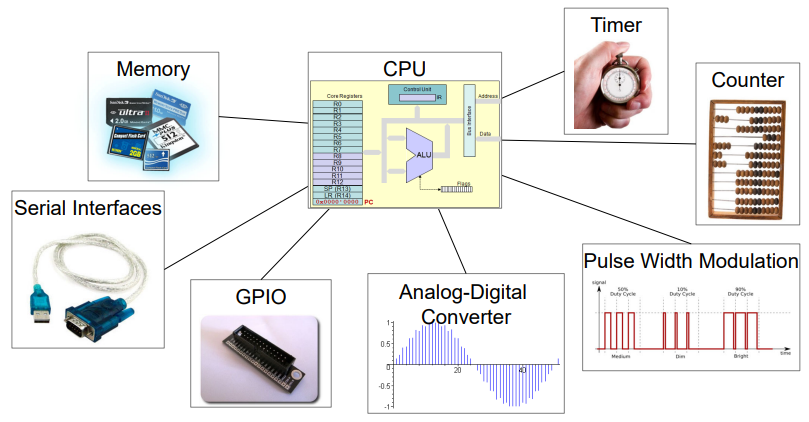
\includegraphics[width=\linewidth]{single_chip_solution.png}
    \\
    before and after an image, we need to add a new line manually. 
\end{definition}




